% =========================================================
% Chapter 3 - System Architecture
% Project: AITasker
%
% Yêu cầu trong main.tex:
% \usepackage{graphicx}
% \usepackage{float}
% \usepackage{longtable}
% \usepackage{array}
% \usepackage{booktabs}
% \graphicspath{{figures/}}
%
% Tên hình được sử dụng đúng theo thư mục figures:
%   architecture.png
%   Context Diagram.png
%   Component Diagram.png
%   Deployment Diagram.png
% =========================================================

\chapter{Kiến trúc hệ thống}
\label{chap:system-architecture}

\section{Giới thiệu}
\label{sec:architecture-introduction}

Chương này mô tả kiến trúc tổng thể của hệ thống AITasker, cách các thành phần được tổ chức, phương thức giao tiếp giữa frontend, backend, cơ sở dữ liệu và các dịch vụ bên ngoài. Kiến trúc được thiết kế theo hướng phân tầng và module hóa nhằm tăng khả năng bảo trì, mở rộng, kiểm thử và tái sử dụng.

AITasker được xây dựng dưới dạng ứng dụng web theo mô hình Client--Server. ReactJS đảm nhiệm giao diện người dùng, FastAPI cung cấp REST API và xử lý nghiệp vụ, trong khi PostgreSQL lưu trữ dữ liệu lâu dài. Hệ thống còn tích hợp cổng thanh toán, dịch vụ email và nền tảng lưu trữ tệp trên cloud.

Các mục tiêu chính của kiến trúc gồm:

\begin{itemize}
    \item Tách biệt rõ giao diện, nghiệp vụ và dữ liệu.
    \item Giảm sự phụ thuộc giữa các module.
    \item Hỗ trợ phân quyền theo vai trò.
    \item Cho phép tích hợp dịch vụ bên ngoài.
    \item Hỗ trợ triển khai trên môi trường cloud.
    \item Tạo nền tảng để mở rộng hệ thống trong tương lai.
\end{itemize}

\section{Nguyên tắc thiết kế kiến trúc}
\label{sec:architecture-principles}

Kiến trúc của AITasker tuân theo các nguyên tắc sau:

\begin{enumerate}
    \item \textbf{Phân tách trách nhiệm:} mỗi lớp đảm nhiệm một nhóm nhiệm vụ riêng.
    \item \textbf{Module hóa:} các chức năng lớn được chia thành các module độc lập.
    \item \textbf{Giao tiếp qua API:} frontend và backend trao đổi dữ liệu bằng REST API và JSON.
    \item \textbf{Bảo mật theo vai trò:} hệ thống sử dụng JWT và RBAC để kiểm soát truy cập.
    \item \textbf{Nhất quán dữ liệu:} các thao tác phức tạp được thực hiện trong transaction.
    \item \textbf{Khả năng thay thế dịch vụ:} email, thanh toán và lưu trữ được tích hợp qua API.
    \item \textbf{Khả năng mở rộng:} kiến trúc hỗ trợ bổ sung module hoặc tách service khi cần.
\end{enumerate}

\section{Kiến trúc tổng thể}
\label{sec:overall-architecture}

AITasker được tổ chức theo kiến trúc phân tầng gồm:

\begin{itemize}
    \item \textbf{Presentation Layer}
    \item \textbf{API Layer}
    \item \textbf{Business Service Layer}
    \item \textbf{Data Access Layer}
    \item \textbf{Infrastructure Layer}
\end{itemize}

\begin{figure}[H]
    \centering
    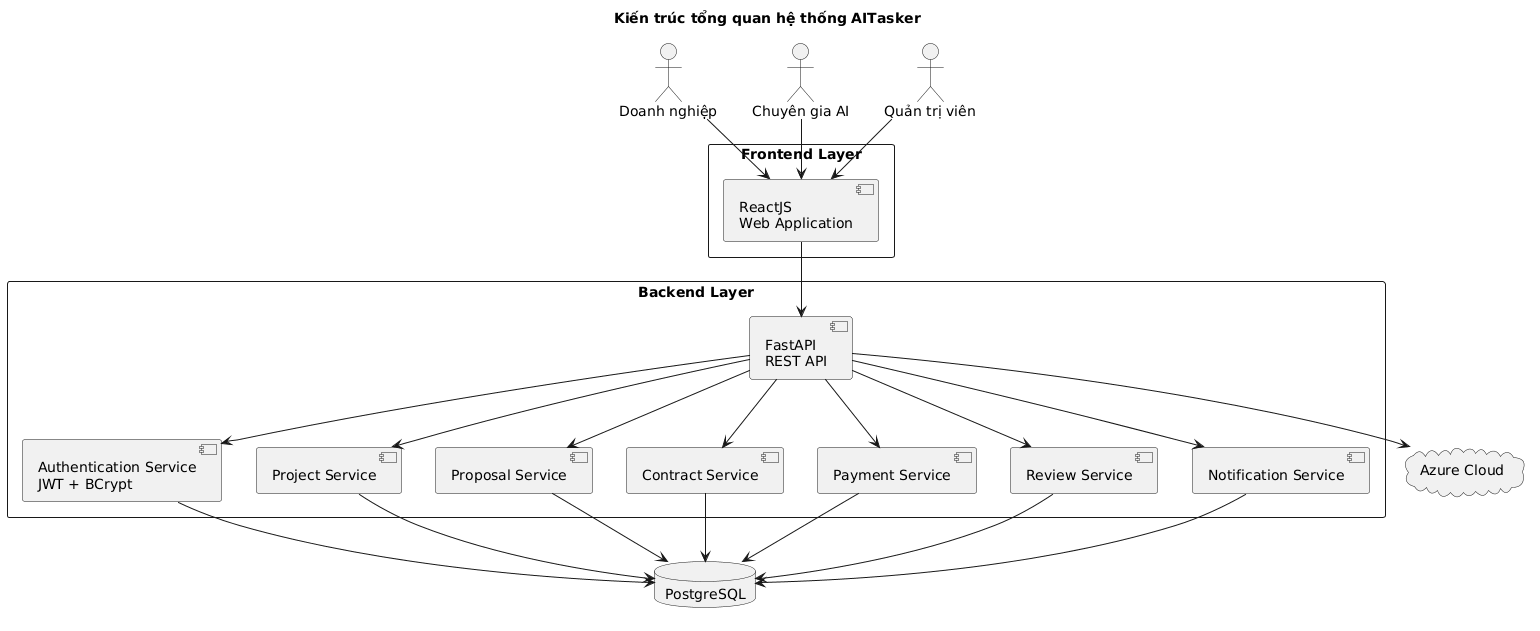
\includegraphics[width=\textwidth]{architecture.png}
    \caption{Kiến trúc tổng thể của hệ thống AITasker}
    \label{fig:architecture-overview}
\end{figure}

Hình~\ref{fig:architecture-overview} mô tả ba nhóm người dùng gồm Doanh nghiệp, Chuyên gia AI và Quản trị viên truy cập ứng dụng ReactJS. Frontend gửi yêu cầu đến FastAPI REST API. Backend xử lý nghiệp vụ thông qua các service và lưu dữ liệu vào PostgreSQL. Các chức năng lưu tệp, gửi email và thanh toán được thực hiện thông qua dịch vụ bên ngoài.

\subsection{Presentation Layer}

Presentation Layer được phát triển bằng ReactJS và chịu trách nhiệm:

\begin{itemize}
    \item Hiển thị giao diện người dùng.
    \item Tiếp nhận thao tác và dữ liệu đầu vào.
    \item Kiểm tra dữ liệu cơ bản phía client.
    \item Gửi request đến backend.
    \item Hiển thị response và thông báo lỗi.
    \item Điều hướng người dùng theo vai trò.
\end{itemize}

Các giao diện chính gồm:

\begin{itemize}
    \item Đăng ký và đăng nhập.
    \item Hồ sơ doanh nghiệp và chuyên gia.
    \item Danh sách và chi tiết dự án.
    \item Proposal.
    \item Hợp đồng và milestone.
    \item Thanh toán.
    \item Nhắn tin và thông báo.
    \item Đánh giá.
    \item Dashboard và trang quản trị.
\end{itemize}

\subsection{API Layer}

API Layer được xây dựng bằng FastAPI. Lớp này thực hiện:

\begin{itemize}
    \item Định nghĩa endpoint REST.
    \item Nhận request và trả response JSON.
    \item Kiểm tra schema bằng Pydantic.
    \item Xác thực JWT.
    \item Kiểm tra quyền truy cập.
    \item Chuyển yêu cầu đến service tương ứng.
    \item Chuyển exception thành mã lỗi HTTP phù hợp.
\end{itemize}

\subsection{Business Service Layer}

Business Service Layer chứa các quy tắc nghiệp vụ chính của hệ thống:

\begin{itemize}
    \item Authentication Service.
    \item User Service.
    \item Enterprise Service.
    \item Expert Service.
    \item Category Service.
    \item Project Service.
    \item Proposal Service.
    \item Contract Service.
    \item Milestone Service.
    \item Payment Service.
    \item Review Service.
    \item Notification Service.
    \item Conversation Service.
    \item Upload Service.
    \item Statistics Service.
\end{itemize}

\subsection{Data Access Layer}

Data Access Layer sử dụng SQLAlchemy ORM để:

\begin{itemize}
    \item Ánh xạ model Python với bảng PostgreSQL.
    \item Thực hiện CRUD.
    \item Quản lý transaction.
    \item Hỗ trợ truy vấn phân trang, tìm kiếm và lọc.
    \item Đảm bảo ràng buộc khóa chính và khóa ngoại.
    \item Phối hợp với Alembic để quản lý migration.
\end{itemize}

\subsection{Infrastructure Layer}

Infrastructure Layer gồm:

\begin{itemize}
    \item Dịch vụ email.
    \item Dịch vụ lưu trữ cloud.
    \item Cổng thanh toán.
    \item Logging và monitoring.
    \item Biến môi trường và quản lý cấu hình.
\end{itemize}

\section{Context Diagram}
\label{sec:context-diagram}

Context Diagram thể hiện AITasker như một hệ thống trung tâm và mô tả luồng tương tác với các tác nhân và hệ thống bên ngoài.

\begin{figure}[H]
    \centering
    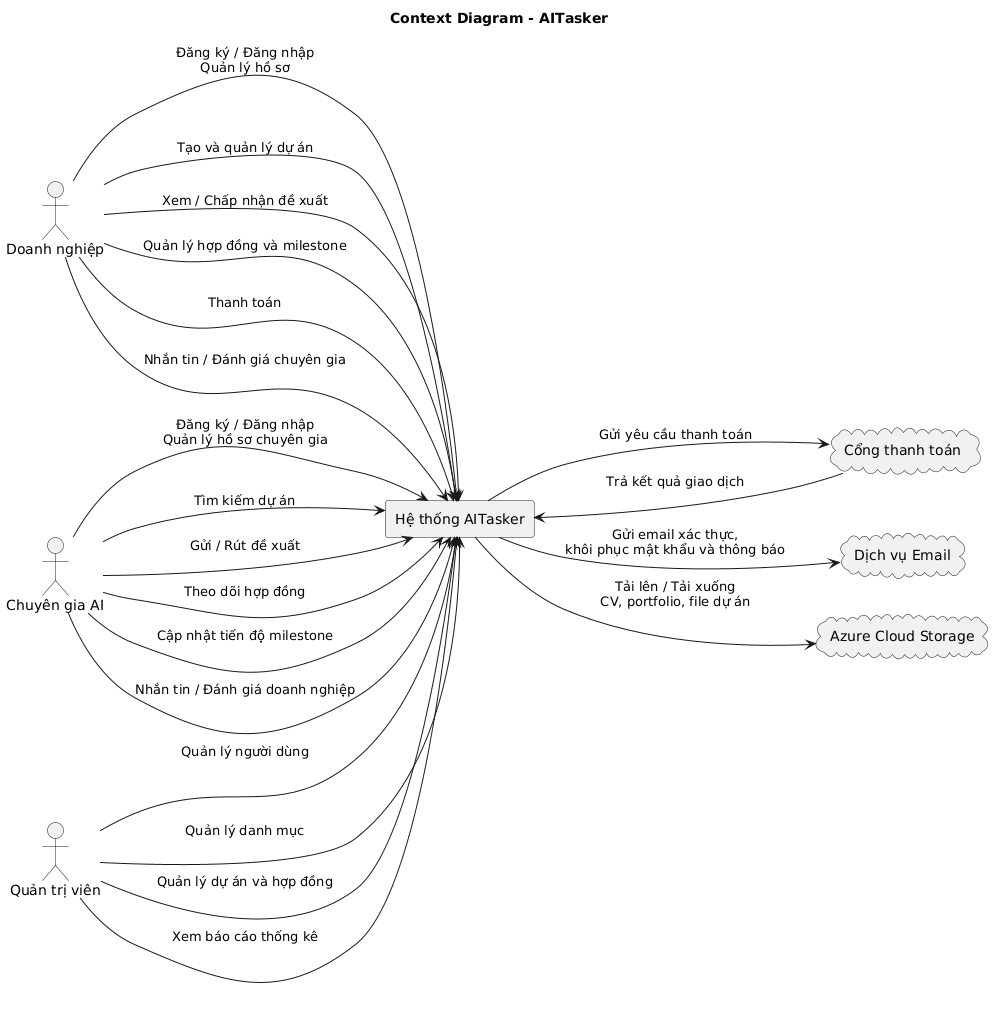
\includegraphics[width=\textwidth]{Context Diagram.png}
    \caption{Context Diagram của hệ thống AITasker}
    \label{fig:context-diagram}
\end{figure}

\subsection{Doanh nghiệp}

Doanh nghiệp sử dụng hệ thống để:

\begin{itemize}
    \item Đăng ký, đăng nhập và quản lý hồ sơ.
    \item Tạo và quản lý dự án.
    \item Xem, chấp nhận hoặc từ chối proposal.
    \item Quản lý hợp đồng và milestone.
    \item Thanh toán.
    \item Nhắn tin với chuyên gia.
    \item Đánh giá chuyên gia.
\end{itemize}

\subsection{Chuyên gia AI}

Chuyên gia sử dụng hệ thống để:

\begin{itemize}
    \item Quản lý hồ sơ, kỹ năng, CV và portfolio.
    \item Tìm kiếm dự án.
    \item Gửi hoặc rút proposal.
    \item Theo dõi hợp đồng.
    \item Cập nhật tiến độ milestone.
    \item Nhắn tin với doanh nghiệp.
    \item Theo dõi thanh toán.
    \item Đánh giá doanh nghiệp.
\end{itemize}

\subsection{Quản trị viên}

Quản trị viên có thể:

\begin{itemize}
    \item Quản lý tài khoản người dùng.
    \item Quản lý danh mục.
    \item Theo dõi dự án và hợp đồng.
    \item Quản lý review hoặc nội dung vi phạm.
    \item Xem báo cáo và thống kê hệ thống.
\end{itemize}

\subsection{Các hệ thống bên ngoài}

\begin{itemize}
    \item \textbf{Cổng thanh toán:} xử lý giao dịch và trả kết quả.
    \item \textbf{Dịch vụ Email:} gửi email xác thực, khôi phục mật khẩu và thông báo.
    \item \textbf{Azure Cloud Storage:} lưu CV, portfolio, avatar và tài liệu dự án.
\end{itemize}

\section{Component Diagram}
\label{sec:component-diagram}

Component Diagram mô tả các module chính trong ứng dụng và mối liên hệ giữa chúng.

\begin{figure}[H]
    \centering
    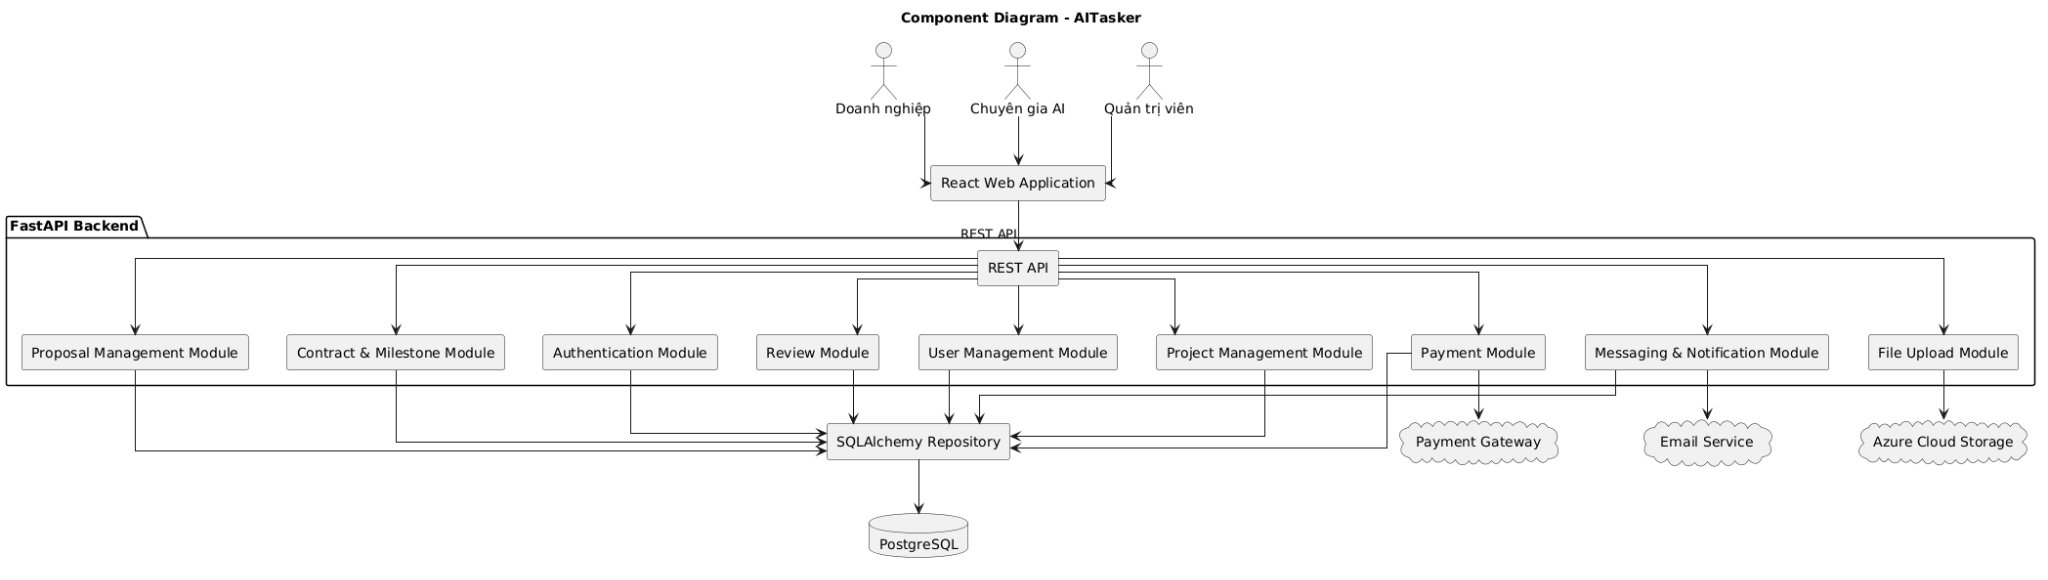
\includegraphics[width=\textwidth]{Component Diagram.png}
    \caption{Component Diagram của hệ thống AITasker}
    \label{fig:component-diagram}
\end{figure}

\subsection{React Web Application}

React Web Application là thành phần giao diện chính, tiếp nhận thao tác của người dùng và gọi REST API.

\subsection{REST API}

REST API là cổng vào của backend. Thành phần này nhận request, xác thực, kiểm tra dữ liệu và chuyển yêu cầu đến module nghiệp vụ.

\subsection{Authentication Module}

Authentication Module xử lý:

\begin{itemize}
    \item Đăng ký và đăng nhập.
    \item Băm và kiểm tra mật khẩu.
    \item Tạo và xác minh JWT.
    \item Đổi và đặt lại mật khẩu.
    \item Phân quyền người dùng.
\end{itemize}

\subsection{User Management Module}

Module này quản lý tài khoản, vai trò, trạng thái hoạt động và thông tin hồ sơ.

\subsection{Project Management Module}

Module này quản lý dự án, danh mục, ngân sách, deadline, tệp đính kèm và trạng thái dự án.

\subsection{Proposal Management Module}

Module này quản lý các thao tác gửi, cập nhật, rút, chấp nhận và từ chối proposal.

\subsection{Contract and Milestone Module}

Module này quản lý hợp đồng, milestone, tiến độ, nghiệm thu và trạng thái thực hiện.

\subsection{Payment Module}

Payment Module tạo giao dịch, gọi cổng thanh toán, lưu kết quả và xử lý hoàn tiền nếu cần.

\subsection{Review Module}

Review Module kiểm tra điều kiện đánh giá, lưu rating và bình luận, đồng thời cập nhật điểm trung bình.

\subsection{Messaging and Notification Module}

Module này hỗ trợ nhắn tin giữa doanh nghiệp và chuyên gia, đồng thời tạo thông báo cho các sự kiện quan trọng.

\subsection{File Upload Module}

Module này kiểm tra định dạng, kích thước và quyền truy cập trước khi lưu tệp lên Azure Cloud Storage.

\subsection{SQLAlchemy Repository}

SQLAlchemy Repository cung cấp lớp truy cập dữ liệu thống nhất cho các module và kết nối đến PostgreSQL.

\section{Deployment Diagram}
\label{sec:deployment-diagram}

Deployment Diagram mô tả cách các thành phần phần mềm được triển khai trên môi trường thực tế.

\begin{figure}[H]
    \centering
    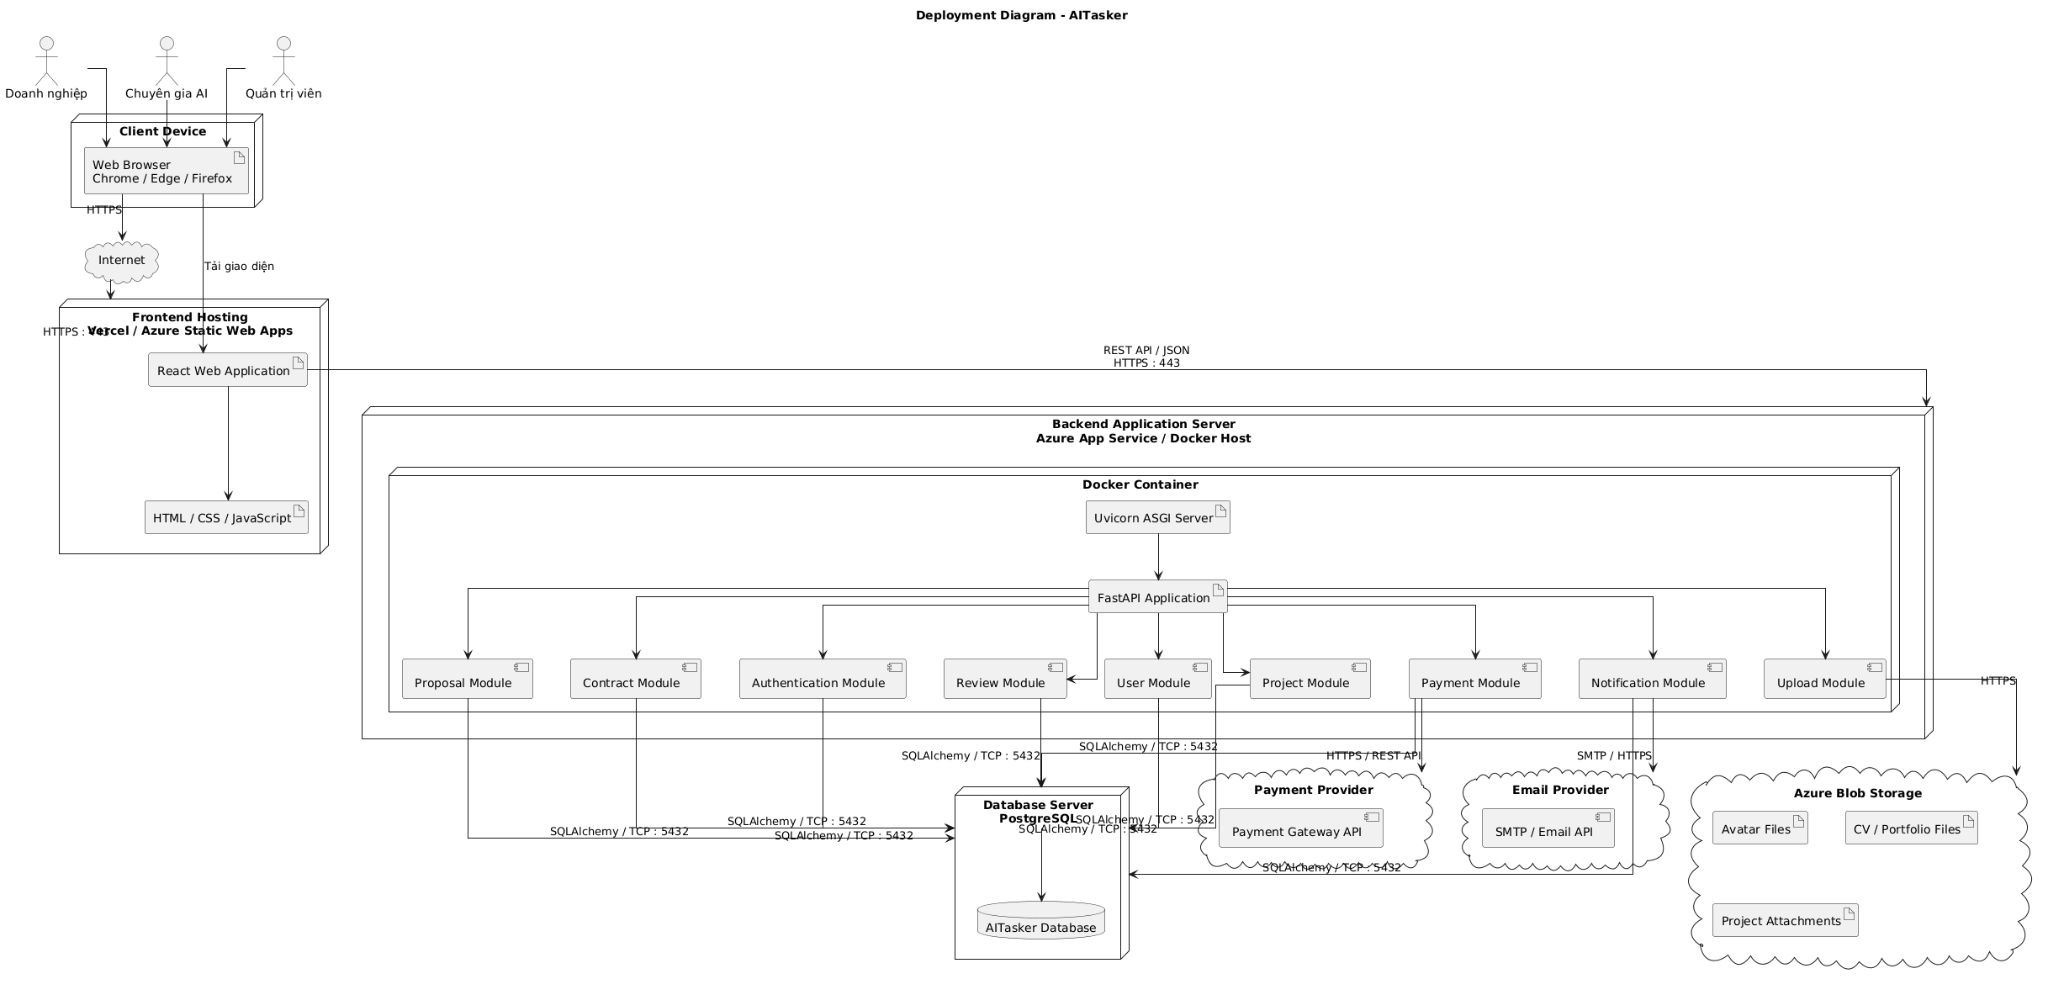
\includegraphics[width=\textwidth]{Deployment Diagram.png}
    \caption{Deployment Diagram của hệ thống AITasker}
    \label{fig:deployment-diagram}
\end{figure}

\subsection{Client Device}

Người dùng truy cập AITasker bằng trình duyệt web như Chrome, Edge hoặc Firefox. Trình duyệt tải giao diện và gửi request qua HTTPS.

\subsection{Frontend Hosting}

Frontend có thể được triển khai trên Vercel, Azure Static Web Apps hoặc máy chủ web tương đương. Node này cung cấp các tệp HTML, CSS và JavaScript.

\subsection{Backend Application Server}

Backend chạy FastAPI trên Uvicorn ASGI Server. Ứng dụng có thể được đóng gói trong Docker Container và triển khai trên Azure App Service hoặc máy chủ Linux.

\subsection{Database Server}

PostgreSQL lưu trữ dữ liệu của toàn bộ hệ thống. Kết nối cơ sở dữ liệu sử dụng SQLAlchemy và được cấu hình thông qua biến môi trường.

\subsection{Payment Provider}

Payment Provider tiếp nhận yêu cầu thanh toán từ Payment Module và trả kết quả giao dịch.

\subsection{Email Provider}

Email Provider tiếp nhận yêu cầu gửi email qua SMTP hoặc HTTPS API.

\subsection{Azure Blob Storage}

Azure Blob Storage lưu trữ:

\begin{itemize}
    \item Avatar.
    \item CV và portfolio.
    \item Tài liệu đính kèm của dự án.
\end{itemize}

\section{Luồng xử lý yêu cầu}
\label{sec:request-flow}

Một yêu cầu điển hình được xử lý theo trình tự:

\begin{enumerate}
    \item Người dùng thao tác trên giao diện ReactJS.
    \item Frontend kiểm tra dữ liệu cơ bản.
    \item Frontend gửi HTTP request đến FastAPI.
    \item FastAPI xác thực JWT và kiểm tra quyền.
    \item Pydantic kiểm tra dữ liệu đầu vào.
    \item Router chuyển request đến service.
    \item Service xử lý quy tắc nghiệp vụ.
    \item SQLAlchemy truy cập PostgreSQL.
    \item Transaction được commit hoặc rollback.
    \item Backend trả response JSON.
    \item Frontend cập nhật giao diện.
\end{enumerate}

\section{Giao tiếp giữa các thành phần}
\label{sec:component-communication}

\begin{longtable}{|p{3.5cm}|p{3.8cm}|p{2.8cm}|p{4.2cm}|}
\caption{Giao tiếp giữa các thành phần}
\label{tab:component-communication} \\ \hline
\textbf{Nguồn} & \textbf{Đích} & \textbf{Giao thức} & \textbf{Mục đích} \\ \hline
\endfirsthead
\hline
\textbf{Nguồn} & \textbf{Đích} & \textbf{Giao thức} & \textbf{Mục đích} \\ \hline
\endhead

Trình duyệt & Frontend Hosting & HTTPS & Tải ứng dụng web. \\ \hline
React Web Application & FastAPI Backend & HTTPS/REST/JSON & Gửi và nhận dữ liệu nghiệp vụ. \\ \hline
FastAPI Backend & PostgreSQL & TCP/SQL & Truy vấn và cập nhật dữ liệu. \\ \hline
FastAPI Backend & Azure Blob Storage & HTTPS & Tải lên và tải xuống tệp. \\ \hline
FastAPI Backend & Email Provider & SMTP hoặc HTTPS & Gửi email. \\ \hline
FastAPI Backend & Payment Provider & HTTPS/REST & Xử lý giao dịch. \\ \hline
\end{longtable}

\section{Kiến trúc bảo mật}
\label{sec:security-architecture}

Các cơ chế bảo mật chính gồm:

\begin{itemize}
    \item Mật khẩu được băm bằng BCrypt.
    \item JWT được dùng để xác thực request.
    \item RBAC giới hạn quyền theo vai trò.
    \item Các endpoint nhạy cảm yêu cầu xác thực.
    \item Giao tiếp trên môi trường triển khai sử dụng HTTPS.
    \item Tệp tải lên được kiểm tra định dạng và kích thước.
    \item Dữ liệu đầu vào được kiểm tra bằng Pydantic.
    \item SQLAlchemy ORM giúp giảm nguy cơ SQL Injection.
    \item Thông tin bí mật được lưu qua biến môi trường.
    \item Các thao tác quan trọng cần được ghi log.
\end{itemize}

\section{Quản lý lỗi và transaction}
\label{sec:error-transaction}

Hệ thống sử dụng các mã lỗi HTTP phù hợp:

\begin{itemize}
    \item HTTP 400 hoặc 422 cho lỗi dữ liệu đầu vào.
    \item HTTP 401 khi chưa xác thực.
    \item HTTP 403 khi không đủ quyền.
    \item HTTP 404 khi không tìm thấy tài nguyên.
    \item HTTP 409 khi xảy ra xung đột dữ liệu.
    \item HTTP 500 cho lỗi máy chủ.
\end{itemize}

Các nghiệp vụ như chấp nhận proposal, tạo hợp đồng, chuyển trạng thái dự án và từ chối proposal còn lại phải được xử lý trong cùng một transaction. Nếu một thao tác thất bại, toàn bộ thay đổi phải được rollback.

\section{Khả năng mở rộng và bảo trì}
\label{sec:scalability-maintainability}

Kiến trúc hiện tại cho phép:

\begin{itemize}
    \item Bổ sung hệ thống gợi ý chuyên gia.
    \item Phát triển ứng dụng di động dùng chung REST API.
    \item Bổ sung chatbot hỗ trợ.
    \item Tách Payment hoặc Notification thành microservice.
    \item Bổ sung cache.
    \item Bổ sung message queue cho tác vụ nền.
    \item Triển khai nhiều backend instance.
    \item Thay thế nhà cung cấp email, payment hoặc storage.
\end{itemize}

\section{Công nghệ sử dụng}
\label{sec:technology-stack}

\begin{table}[H]
    \centering
    \caption{Công nghệ sử dụng trong hệ thống AITasker}
    \label{tab:technology-stack}
    \begin{tabular}{|p{4.4cm}|p{9.0cm}|}
        \hline
        \textbf{Thành phần} & \textbf{Công nghệ} \\ \hline
        Frontend & ReactJS, HTML, CSS, JavaScript hoặc TypeScript \\ \hline
        Backend & Python 3.12, FastAPI, Uvicorn \\ \hline
        Validation & Pydantic v2 \\ \hline
        ORM & SQLAlchemy \\ \hline
        Migration & Alembic \\ \hline
        Database & PostgreSQL \\ \hline
        Authentication & JWT \\ \hline
        Password security & BCrypt \\ \hline
        Storage & Azure Blob Storage \\ \hline
        Email & SMTP hoặc Email API \\ \hline
        Payment & Payment Gateway API \\ \hline
        Version control & Git và GitHub \\ \hline
        Development environment & Visual Studio Code \\ \hline
        Diagramming & PlantUML và Draw.io \\ \hline
    \end{tabular}
\end{table}

\section{Ưu điểm và hạn chế}
\label{sec:architecture-evaluation}

\subsection{Ưu điểm}

\begin{itemize}
    \item Kiến trúc rõ ràng và dễ hiểu.
    \item Dễ kiểm thử theo module.
    \item Dễ bảo trì và mở rộng.
    \item Phù hợp với quy mô đồ án.
    \item Có thể triển khai trên cloud.
    \item Hỗ trợ tích hợp dịch vụ bên ngoài.
\end{itemize}

\subsection{Hạn chế}

\begin{itemize}
    \item Backend modular monolith có thể lớn khi số lượng chức năng tăng.
    \item Khả năng xử lý thời gian thực cần bổ sung WebSocket hoặc message broker.
    \item Tính sẵn sàng phụ thuộc vào cấu hình database và dịch vụ ngoài.
    \item Việc chuyển sang microservice sẽ cần thêm cơ chế quản lý phân tán.
\end{itemize}

\section{Kết luận}
\label{sec:architecture-conclusion}

Kiến trúc AITasker được xây dựng theo mô hình Client--Server, kết hợp kiến trúc phân tầng và module hóa. ReactJS đảm nhiệm giao diện, FastAPI xử lý REST API và nghiệp vụ, SQLAlchemy cung cấp lớp truy cập dữ liệu, còn PostgreSQL lưu trữ dữ liệu hệ thống. Các dịch vụ thanh toán, email và lưu trữ được tích hợp như những thành phần bên ngoài.

Kiến trúc này đáp ứng phạm vi hiện tại của đồ án, đồng thời tạo cơ sở để phát triển thêm hệ thống gợi ý, chatbot, ứng dụng di động và mô hình triển khai phân tán trong tương lai.
